A major goal of the thesis was to improve the performance of array-based languages like \matlab and Python's NumPy library by compiling computationally intensive functions to C++. To demonstrate these performance results, we compared the performance of the generated code with that provided by various tools for scientific computing. Seventeen \matlab benchmarks and nine Python benchmarks were used to perform this comparision. Different variations of generated code that can be generated by turning optimisations on and off were also tested. 

In this chapter, we give a brief description of the benchmarks that were used to test the performance followed by the results themselves and our analysis of these results. 
\section{Benchmarks}
Two separate set of benchmarks  were used for \matlab and Python. 
\subsection{\matlab Benchmarks}
The \matlab benchmarks used for the performance were obtained from various sources. The sources include the FALCON project\cite{DeRose:1999} , the OTTER project \cite{quinn}, Chalmers university of technology\footnote{\url{http://www.elmagn.chalmers.se/courses/CEM/}}, Mathworks central file exchange\footnote{\url{http://www.mathworks.com/matlabcentral/fileexchange}} and the presentation on parallel programming in \matlab by Burkhadt and Cliff\footnote{\url{http://people.sc.fsu.edu/~jburkardt/presentations/matlab_parallel.pdf}}. The benchmarks cover commonly occurring \matlab features such as builtin function calls, array indexing including slicing operations and array operations like array addition, matrix multiplication, etc. Table \ref{tab:matBench} gives the list of benchmarks used along with their descriptions and source.  
\begin{table}[htbp]
\resizebox{\columnwidth}{!}{%
\centering
\begin{tabular}{|c|c|c|}
\hline
Benchmark  & Source               & Description\\
\hhline{|=|=|=|}
bbai       & MATLAB file exchange & Implementation of the Babai estimation algorithm \\
\hline 
bubble       & McLab                & Bubble Sort \\
\hline 
capr       & Chalmers University  & \begin{tabular}{@{} c@{}} Computes the capacitance of a transmission line \\ using fine difference and Gauss-seidel\end{tabular} \\
\hline 
clos       & Otter project        & Calculates the transitive closure of a directed graph \\
\hline 
crni       & Falcon project       & Crank-Nicholson solution to the heat equation \\
\hline
dich       & Falcon project       & Dirichlet solution to Laplace's equation\\
\hline
fiff       & Falcon project       & Computes the finite difference solution to the wave equation \\
\hline
ldgr       &  -                    & Calculates derivatives of Legendre polynomials \\
\hline
mbrt       & McFor project        & Computes Mandelbrot sets \\
\hline
nb1d       & Otter project        & Simulates the 1-dimensional n-body problem \\
\hline
matmul     & McLab                & naive matrix multiplication \\
\hline
mcpi       & McLab                & Calculates $\pi$ by the Monte Carlo method   \\
\hline
numprime   & Burkardt and Cliff   & \begin{tabular}{@{} c@{}} Simulates the sieve of Eratosthenes for  \\calculating number of prime numbers less than a given number \end{tabular} \\
\hline
scra       & ACM CALGO            & \begin{tabular}{@{} c@{}} Implementation to produce a reduced-rank \\ approximation to a matrix \end{tabular}   \\
\hline
spqr       & ACM CALGO            & \begin{tabular}{@{} c@{}} Implementation to compute a pivoted \\ semi-QR decomposition of an m-by-n matrix A \end{tabular} \\
\hline
quadrature & Burkardt and Cliff   &  \begin{tabular}{@{} c@{}} Simulates the quadrature approach \\ for  calculating integral of a function \end{tabular} \\
\hline
\end{tabular}
}
\caption[List of \matlab Benchmarks]{List of \matlab Benchmarks used for experiments}
\label{tab:matBench}
\end{table}
\subsection{Python Benchmarks}
Many of the Python benchmarks are Python ports of the Ostrich benchmark suite\cite{Khan:2014:UJW:2661088.2661090}. The benchmarks contain scalar operations as well as array index operation. Six of the nine Python benchmarks support parallelism. Table \ref{tab:pyBenches} gives the list of Python benchmarks that were used. The Python ports of the Ostrich benchmark suite are known as PyDwarfs. The rest of the benchmarks are part of a suite that were put together by the open-source Python community focused on compilers. The suite is known as NumFocus and can be found  on github\footnote{\url{https://github.com/numfocus/python-benchmarks}}. 
\begin{table}[htbp]
\centering
\begin{tabular}{|c|l|c|}
\hline
Benchmark Name & Source    & Description                                                                                                                                              \\ 
\hhline{|=|=|=|}
arc\_distance  & NumFocus & \begin{tabular}[c]{@{}c@{}} Calculates the pairwise arc distance \\ between all points in vector a and b.\end{tabular} \\ \hline                                                                                                                                                   
fft            & Pydwarfs  & Fast Fourier Transform                                                                                                                                   \\ \hline
growcut        & NumFocus &  Implementation of GrowCut segmentation                                                                                                                                                         \\ \hline
julia          & NumFocus &  Calculates the Julia fractal                                                                                                                                                        \\ \hline
lud            & PyDwarfs  & \begin{tabular}[c]{@{}c@{}}LU decomposition  factors a matrix as the product of a \\ lower triangular matrix and an upper triangular matrix\end{tabular} \\ \hline
pagerank       & PyDwarfs  & PageRank is a link analysis algorithm used by Google Search                                                                                              \\ \hline
pairwise       & NumFocus &   \begin{tabular}[c]{@{}c@{}} Computes the pairwise distance \\ between a set of points in 3D space.\end{tabular}                                                                                                                                                         \\ \hline
spmv           & PyDwarfs  & Sparse Matrix-Vector Multiplication                                                                                                                      \\ \hline
srad           & PyDwarfs  & \begin{tabular}[c]{@{}c@{}}Tracks the movement of a mouse heart over a sequence  of 104\\ 609x590 ultrasound images to record response to the stimulus \end{tabular} 
\\ \hline
\end{tabular}
\caption[List of Python Benchmarks used for experiments]{List of Python Benchmarks used for experiments}
\label{tab:pyBenches}
\end{table}

\section{Experimental Setup}
We ran separate experiments for \matlab and Python benchmarks. Different variations of the code generated by \velocty were also tested. Table \ref{tab:benchvar} gives a list of variations generated by \velocty. All the benchmarks were tested on a machine running GNU/Linux(3.8.0-35-generic \#52-Ubuntu) with a Intel(R) Core(TM) i7-3820 CPU @ 3.60GHz with 16GB of memory. We also ran experiments on different compiler tools developed for both \matlab and Python. Each version of the benchmarks was executed 10 times and the average execution time was recorded. The following subsections describe the tools for each language against which the different versions of \velocty were compared and explain the aspects of the experimental setup that are specific to each language.

\begin{table}[h]
\centering
\begin{tabular}{|c|c|}
\hline
Variation name                                                               & Description                                                                                                                        \\ \hhline{|=|=|}
Baseline VeloCty                                                             & \begin{tabular}[c]{@{}c@{}}Generated C++ code without optimisations and \\ with array bounds checks enabled\end{tabular}           \\ \hline
VeloCty no-checks                                                            & \begin{tabular}[c]{@{}c@{}}Generated C++ code without optimisations and \\ without array bounds checks.\end{tabular}               \\ \hline
VeloCty memory optimisation                                                  & \begin{tabular}[c]{@{}c@{}}Generated C++ code with memory optimisations and \\ with array bounds checks enabled.\end{tabular}      \\ \hline
\begin{tabular}[c]{@{}c@{}}VeloCty bounds check \\ optimisation\end{tabular} & \begin{tabular}[c]{@{}c@{}}Generated C++ code with boundscheck optimisations \\ and with array bounds checks enabled.\end{tabular} \\ \hline
VeloCty parallel                                                             & \begin{tabular}[c]{@{}c@{}}Generated C++ code with parallel constructs \\ and with array bounds checks enabled.\end{tabular}       \\ \hline
VeloCty all optimisations                                                    & \begin{tabular}[c]{@{}c@{}}Generated C++ code with all optimisations\\  and with array bounds checks enabled.\end{tabular}         \\ \hline
\end{tabular}
\caption[List of benchmark variations generated by \velocty]{ The table gives a list of benchmark variations generated by \velocty along with the description of each}
\label{tab:benchvar}
\end{table}

\subsection{Experimental Setup for \matlab}
 In order to gauge \velocty's performance against current compiler tools for \matlab, the \matlab benchmarks were executed on the Mathworks' 2014b release of the \matlab interpreter and JIT compiler. We also used the Mathworks' \matlab-Coder implementation to compile the benchmarks to C++. This generated C++ code is compiled as  a dynamic library similar to the method used by \velocty. Both \velocty and \matlab-coder use the MEX compiler to compile the C++ code and generate the shared library. MEX internally uses the g++-4.6.4 compiler. 
\subsection{Experimental Setup for Python}
 Similar to \matlab, we gauged our performance of the \velocty code against exising compiler tools for Python. We used the reference C-Python interpreter version 3.2.3  and Cython\cite{cython} version 0.21, which is a compiler used to generate C-extensions for Python. Both, \velocty and Cython use g++-4.6.4 through distutils for compilation. 

\section{\matlab Results}

\subsection{Overall Results}
We ran experiments on 17 \matlab benchmarks. We compared the VeloCty with all optimisations enabled  with the Mathworks' \matlab implementation and \matlab-coder. We measured the speedup of the VeloCty backend and the \matlab-coder versions compared to Mathwork's \matlab JIT compiler. Figure \ref{fig:results_cwochecks} shows a bar graph with the results of the experiment. The red bars show the speedup of \matlab-coder and the blue bars show the speedup of the VeloCty backend with all optimisations enabled. The geometric mean for the speedup of the VeloCty version was 8.05x as compared to the geometric mean of 3.89x for the \matlab-coder version. The largest speedup was shown by the quadrature benchmark. The benchmark was 458x times faster than Mathworks' \matlab. The benchmark consists of operations on scalar operations and hence gives a high speedup. The smallest speedup of 1.31x, is given by the closure benchmark. The benchmark's computationally intensive code section is a while loop containing a matrix multiplication operation. All three versions, the VeloCty backend, Mathwork's \matlab and \matlab-coder use the Intel MKL BLAS library and hence show similiar performance. 

\begin{figure}[htbp]
\centering
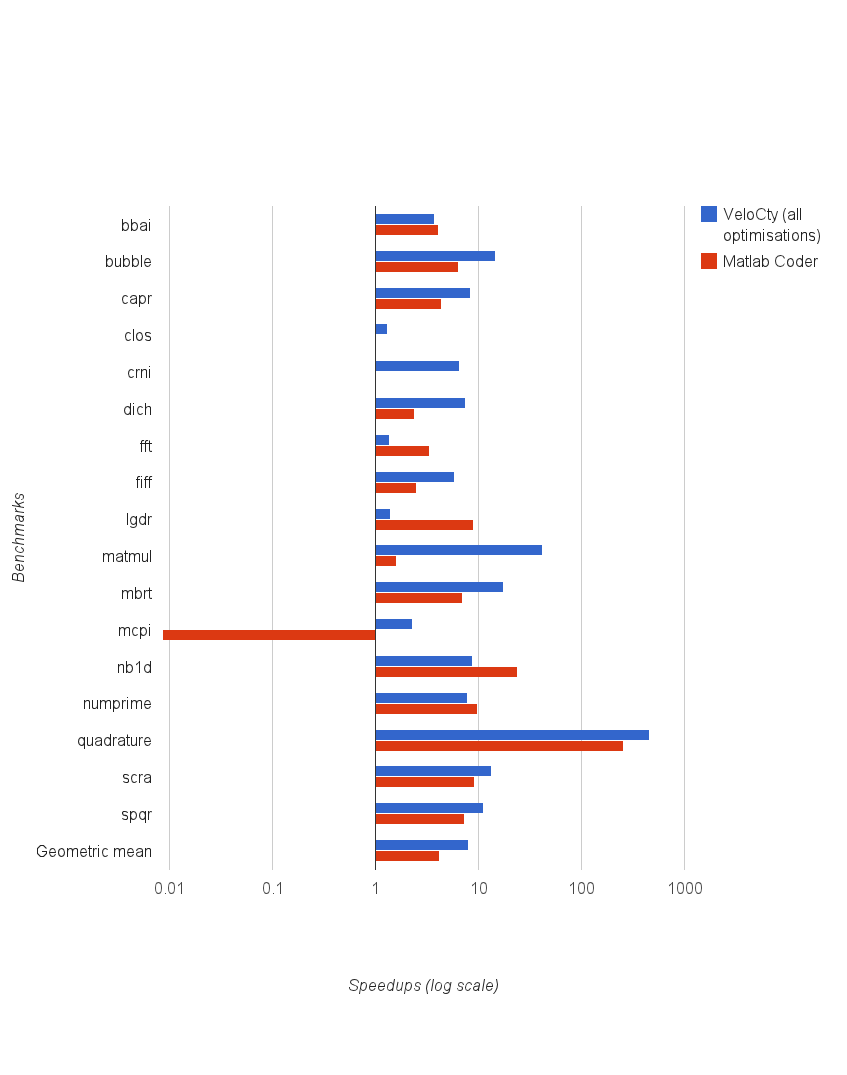
\includegraphics[scale=0.5]{Figures/results_cwochecks.png}
\caption[Experiment results for the baseline \velocty backend for \matlab benchmarks]{The bar graph gives the speedups of the \velocty backend with all optimisations enabled and \matlab-coder compared to the Mathworks' JIT and VM implemenation. Higher is better }
\label{fig:results_cwochecks}
\end{figure}

For most benchmarks, our VeloCty backend was faster than \matlab-coder. The benchmarks, \textsf{bbai}, \textsf{lgdr}, \textsf{nb1d}, \textsf{fft} and \textsf{numprime} are exceptions. \textsf{Lgdr} \textsf{bbai} and \textsf{nb1d} contain array slicing and array operations which do not internally make calls to the BLAS library and hence take longer to execute compared to \matlab-coder. The \textsf{fft} benchmark contains a loop whose direction can not be identified at run time and hence a loop vector needs to be initialised and iterated over as described in Subsection \ref{subsec:forStmt}. \textsf{numprime} contains scalar operations and a square root function call. The square root function's \matlab implementation may be faster than the standard C++ implementation and hence the \textsf{numprime} benchmark performs in \matlab-coder than in the \velocty version. 

As we can also observe, \matlab-coder shows a positive speedup on all benchmarks except for \textsf{mcpi}. The reason for this is that the benchmark contains a loop with calls to the random function inside the body. These functions return a single scalar value. However, in case of \matlab-coder, an 1x1 matrix is returned. Since a heap allocation is needed for every iteration, the benchmark is significantly slower than Mathworks' \matlab. 

The \textsf{crni} benchmark is an example of a feature that is supported by \velocty but not by \matlab-coder. The benchmark contains a growing array which is not supported by \matlab-coder. Hence, a \matlab-coder version of the benchmark cannot be generated. 

\subsection{Impact of Array Bounds Checks on Performance}
Table \ref{tab:CwovsCw} gives the slowdown of the generated VeloCty code because of bounds checks. This experiment allowed us to determine the effect bounds check had on performance. The table lists the slowdown of the baseline \velocty code compared to the \velocty code with checks disabled. 6 benchmarks show a slowdown of 1.5x or higher. These benchmarks are \textsf{bubble}, \textsf{capr}, \textsf{dich}, \textsf{fft}, \textsf{fiff} and \textsf{matmul}. The geometric mean of the slowdown for all benchmarks is 1.66x. If only the geometric mean of the  6 benchmarks that slowed down significantly  are considered, we get a geometric mean of 3.66x. The matmul benchmark shows the highest slowdown with 10.44x. The slowdown for the \textsf{crni} benchmark cannot be calculated since a version of the generated code without checks cannot be executed. 

\begin{table}[htbp]
\centering
\begin{tabular}{|c|c|}
\hline
Benchmarks                           & Slowdown     \\ \hhline{|=|=|}
bbai                                 & 1.21  \\ \hline
bubble                               & 8.61  \\ \hline
capr                                 & 2.62   \\ \hline
clos                                 & 0.84 \\ \hline
crni                                 & -            \\ \hline
dich                                 & 1.71\\ \hline
fft                                  & 1.43\\ \hline
fiff                                 & 4.15\\ \hline
lgdr                                 & 1.01\\ \hline
matmul                               & 10.44\\ \hline
mbrt                                 & 1.02\\ \hline
mcpi                                 & 1.00\\ \hline
nb1d                                 & 1.05\\ \hline
numprime                             & 1.06\\ \hline
quadrature                           & 1.00\\ \hline
scra                                 & 1.99\\ \hline
spqr                                 & 1.04\\ \hline
Geometric mean                       & 1.66\\ \hline
Geometric mean (Affected Benchmarks) & 3.66\\ \hline
\end{tabular}
\caption[Slowdown of \velocty with checks enabled]{The table lists the slowdowns of the  VeloCty baseline code  compared to when \velocty-no-checks}
\label{tab:CwovsCw}
\end{table}
\subsection{Impact of Bounds Check Optimisations on Performance}
The previous experiment showed us that bounds checks have a significant impact on performance. This was the reason we implemented an optmisation to elminate the bounds checks where possible. In order to determine the improvement in performance when bounds check optimisations were enabled, we compared the speedup of the generated VeloCty code with bounds check optimisation enabled  against the baseline \velocty version. Table \ref{tab:CwvsCbc} gives the speedups for all the benchmarks. The geometric mean of speedups with the optimisation enabled is 1.62x. If the speedups of the benchmarks that show a significant speedup are considered, we see a speedup of 3.18x. The \textsf{fft} benchmark does not show an improvement in performance. This is because the benchmark contains a loop whose direction can not be determined and hence the bounds checks inside the loop body  can not be moved outside.
\begin{table}[h]
\centering
\begin{tabular}{|c|c|}
\hline
Benchmarks     & Speedups \\ \hhline{|=|=|}
bbai           & 1.07     \\ \hline
bubble         & 7.84     \\ \hline
capr           & 2.49     \\ \hline
clos           & 1.00     \\ \hline
crni           & 2.23     \\ \hline
dich           & 1.71     \\ \hline
fft            & 1.01     \\ \hline
fiff           & 4.12     \\ \hline
lgdr           & 1.02     \\ \hline
matmul         & 10.54    \\ \hline
mbrt           & 1.00     \\ \hline
mcpi           & 1.00     \\ \hline
nb1d           & 1.06     \\ \hline
numprime       & 0.99     \\ \hline
quadrature     & 1.00     \\ \hline
scra           & 1.04     \\ \hline
spqr           & 1.01     \\ \hline
Geometric mean & 1.62     \\ \hline
\end{tabular}
\caption[Speedup of \velocty with bounds check optimisation turned on]{The table lists the speedups obtained when the array bounds check optimisations are turned on against the baseline \velocty code}
\label{tab:CwvsCbc}
\end{table}
\subsection{Impact of Memory Optimisations on Performance}
As we had already identified that many of the benchmarks contain array operations inside a loop where memory is allocated continuously. As dynamic memory allocations are expensive, we implemented an optmisation to eliminate unecessary memory allocations and instead reuse previously allocated memory where possible. The performance improvement of the generated code when the memory optimisations were enabled was also gauged. We calculated the speedups of the generated VeloCty code with memory optimisations enabled compared to the baseline VeloCty code for all the benchmarks. Table \ref{tab:cmvscwo} gives the speedups for the benchmarks. The geometric mean of the speedups for all benchmarks is 1.14x. Four benchmarks, \textsf{capr}, \textsf{nb1d}, \textsf{scra}, \textsf{spqr} showed speedups of 1.54x, 1.59x, 3.57x and 2.77x respectively. All of these benchmarks consisted of loops inside which array operations were performed. Since, because of the optimisation, previously allocated memory was reused, we observed a noticeable speedup. The geometric mean of the four affected benchmarks is 2.36x. 
\begin{table}[h]
\centering
\begin{tabular}{|c|c|}
\hline
Benchmarks     & VeloCty Memory optimisation \\ \hhline{|=|=|}
bbai           & 1.18                        \\ \hline
bubble         & 1.00                        \\ \hline
capr           & 1.54                        \\ \hline
clos           & 1.00                        \\ \hline
crni           & 1.10                        \\ \hline
dich           & 1.00                        \\ \hline
fft            & 1.00                        \\ \hline
fiff           & 1.14                        \\ \hline
lgdr           & 1.08                        \\ \hline
matmul         & 0.99                        \\ \hline
mbrt           & 1.00                        \\ \hline
mcpi           & 1.00                        \\ \hline
nb1d           & 1.59                        \\ \hline
numprime       & 1.00                        \\ \hline
quadrature     & 1.00                        \\ \hline
scra           & 3.33                        \\ \hline
spqr           & 2.77                        \\ \hline
Geometric mean & 1.23                        \\ \hline
Geometric mean(Affected Benchmarks)  & 2.36                        \\ \hline
\end{tabular}
\caption[Speedup of \velocty code when memory optimisations are enabled]{The table lists the speedups for the different \matlab benchmarks when memory optimisations are enabled compared to baseline \velocty code}
\label{tab:cmvscwo}
\end{table}
\subsection{Impact of Parallel Execution of \velocty Code}

Three of the \matlab benchmarks, \textsf{nb1d}, \textsf{matmul} and \textsf{mbrt} can be executed in parallel. We calculated the speedups of the three benchmarks in parallel compared to the baseline VeloCty version and the speedups of the benchmarks executed using the Mathworks' Parallel Computing Toolbox\cite{matlabpar} compared to the Mathwork's \matlab JIT executing code sequentially.

 Table \ref{tab:cpvscwo} gives the speedups for the three benchmarks. In the case of the \velocty parallel version, matmul and mbrt benchmarks show significant speedups of 3.87x and 3.26x respectively. This is because in the case of the the two benchmarks, a very small portion of the code needs to be executed sequentially. Moreover, parallel portion of the code is computationally intensive thus making the thread management time a small portion of the total execution time. On the other hand, the nb1d benchmark shows no speedup. The parallel version is 1.01 times faster than the baseline \velocty. This can be attributed to the fact that the loop being parallelised is nested inside another loop executing sequentially. Moreover, the loop being executed in parallel in not computationally intensive and hence the benchmark does not benefit from parallel execution. 

On the other hand, the Parallel Computing Toolbox shows a speedup of 3.35x compared to the sequential \matlab version. This algorithm is embarassingly parallel and has little data transfer which is ideal for the toolbox's multiprocessing based model. The \textsf{matmul} benchmark shows a speedup of 1.05x. The smaller speedup may be attributed to higher number of data transfers. The benchmark \textsf{nb1d} shows a slowdown when executed in parallel which may be because of the fact that since only the inner loop is executed in parallel, the more time is spent in the master process in data management than in code execution. 
\begin{table}[htbp]
\centering
\begin{tabular}{|c|c|c|}
\hline
Benchmarks & \begin{tabular}[c]{@{}c@{}}Speedup Velocty parallel\\ v/s VeloCty Baseline\end{tabular} & \begin{tabular}[c]{@{}c@{}}Speedup \matlab Parallel\\ v/s \matlab Sequential\end{tabular} \\ \hhline{|=|=|=|}
matmul     & 3.87                                                                                    & 1.05                                                                                    \\ \hline
mbrt       & 3.26                                                                                    & 3.35                                                                                    \\ \hline
nb1d       & 1.01                                                                                    & 0.32                                                                                    \\ \hline
\end{tabular}
\caption[Speedup of Generated Code with Parallel constructs]{The table lists the speedups of the benchmarks in VeloCty code with parallel execution over baseline VeloCty code.}
\label{tab:cpvscwo}
\end{table}

\subsection{Summary of \matlab Results}
Figure \ref{fig:results_final} shows a chart with the speedups of the diferent versions of \velocty code for the \matlab benchmarks compared to the Mathworks' \matlab interpreter and VM. The blue bars represent the speedups of baseline \velocty, the red bars indicate the speedups of the \velocty versions with bounds check optimisations turned on, the yellow bars indicate the speedups of the \velocty versions with both memory and bounds check optimisations turned on and the green bars indicate the speedups of the \velocty versions with bounds check optimisation, memory optimisation and parallel code execution. 
\begin{figure}[htbp]
\centering
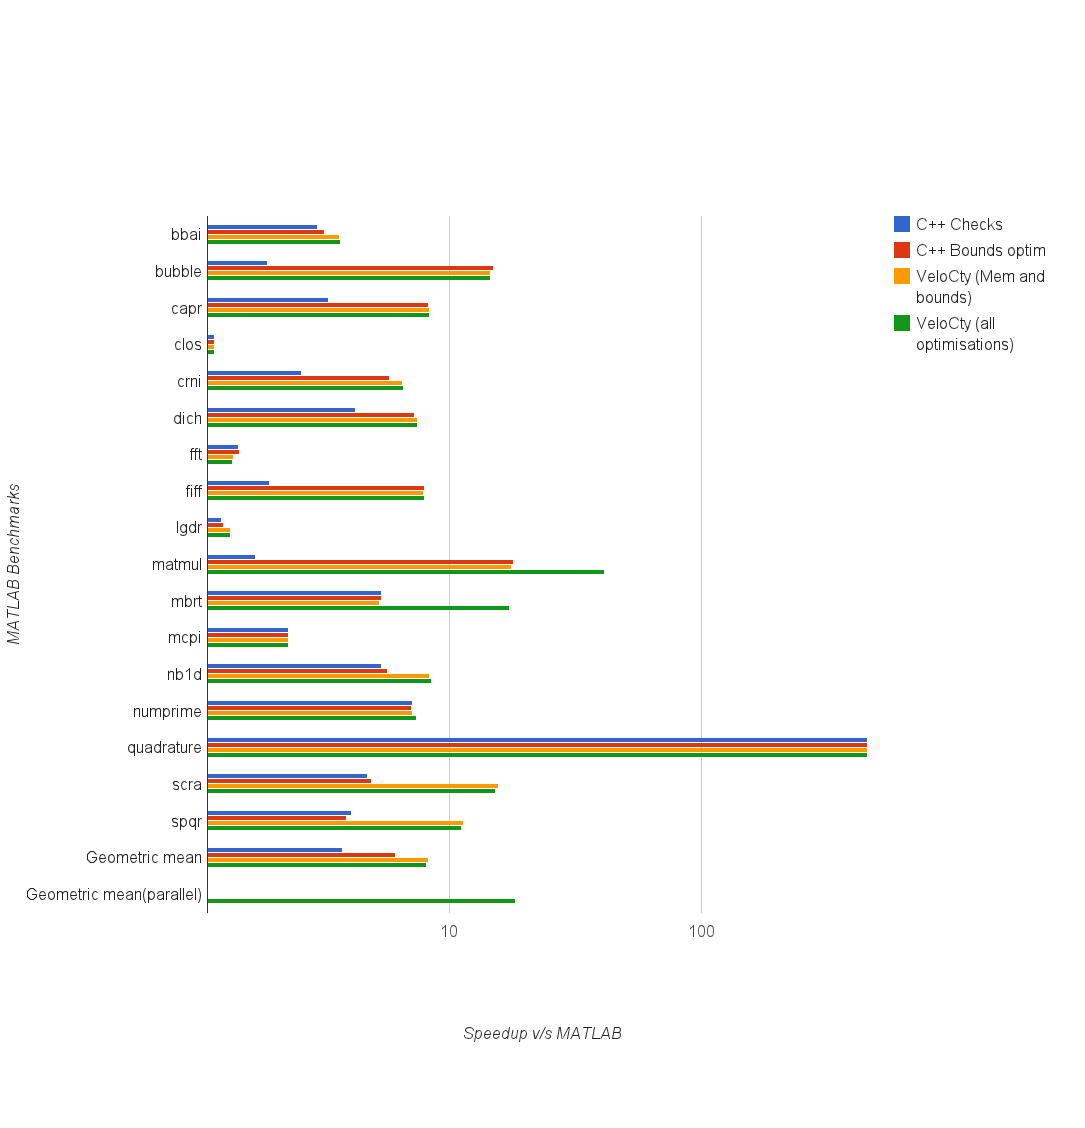
\includegraphics[scale=0.45]{Figures/final_mat.png}
\caption[Summary of \matlab benchmark results]{The figure compares the speedups of different \velocty versions against the Mathworks' interpreter and JIT compiler version for the \matlab benchmarks. Geometric mean(parallel) gives the geometric mean of three benchmarks matmul, mbrt and nb1d when they are executed with all optimisations.}
\label{fig:results_mat}
\end{figure}

As we can observe the we see an increase in the geometric means as we add optimisations. The geometric mean for baseline \velocty is 3.76x, the geomtric mean for the \velocty version with bounds checks optimisations enabled was 6.10x, that for \velocty with bounds checks and memory optimisations was 8.24x and finally the version with all optimisations was 8.5x. In case of the \velocty versions with all the optimisations, if we only consider the three benchmarks that are executed in parallel, we observe a geometric mean of 18.27x.

\section{Python Results}
\subsection{Overall Results}
We ran experiments on 9 Python benchmarks. Similar to the experiments on \matlab benchmarks, we compared the generated VeloCty code without bounds checks to Cython and the CPython interpreter. Figure \ref{fig:results_cwochecks_py} is a bar graph showing the speedup of the generated VeloCty code with checks disabled, the generated VeloCty code with checks enabled and the Cython code compared to the CPython interpreter. The blue bars indicate the speedup of the generated VeloCty code with checks enabled and the red bars indicate the speedup of the Cython code. The geometric mean of the speedups for the generated VeloCty code without checks was 397.17x. The largest speedup of 1281.67x was shown by the \textsf{lud} benchmark. The smallest speedup of 40.98 was shown by the \textsf{fft} benchmark. Note that the Python results are compared against a pure interpreter, C-Python, whereas in case of the \matlab, the results were compared against a interpreter with a JIT compiler. A JIT compiler gives better performance compared to a pure interpreter. Hence we see higher speedups for the \velocty code for Python as compared to the ones we observed for \matlab. 
\begin{figure}[htbp]
\centering
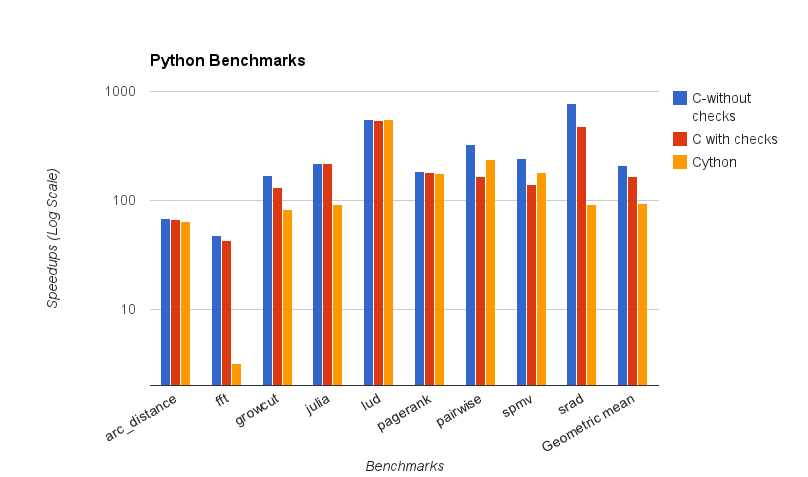
\includegraphics[scale=0.5]{Figures/results_cwochecks_py.png}
\caption{The figure compares the speedups of the \velocty code with all optimisations enabled and and speedups of Cython against the C-Python version for the Python benchmarks.}
\label{fig:results_cwochecks_py}
\end{figure}

The baseline VeloCty code is faster than the Cython code for all the benchmarks. Comparing the speedup of our generated VeloCty code to the Cython code, a mean speedup of 2.21x was found. The largest speedup of 14.93x was shown by the \textsf{fft} benchmark. The benchmarks \textsf{arc\_distance}, \textsf{lud} and \textsf{pagerank} take the same time to execute as our generated C++ code. All three benchmarks have fewer array index operations and more scalar operations compared to the other benchmarks. On the other hand the \textsf{fft} benchmark performs significantly better for the generated VeloCty code than the Cython version. The \textsf{fft} benchmark contains recursive function calls. Cython adds checks to ensure validity of the input arguments of a function as well as validity of the arguments being passed from the function call point. 

\subsection{Impact of Array Bounds Checks on Performance}
Enabling array bounds checks gives a significant slowdown in 4 of the 9 benchmarks. These benchmarks are \textsf{growcut}, \textsf{pairwise}, \textsf{spmv} and \textsf{srad}. Table \ref{tab:cwvscwopy} lists the slowdowns observed for the generated VeloCty versions with checks enabled compared to the generated VeloCty version with checks disabled. The geometric mean of the slowdown is 1.27x. The geometric mean of the slowdown for the affected benchmarks was 1.63. The highest slowdown was shown by the \textsf{pairwise} benchmark. Benchmarks which were not affected by array bounds checks enabled were ones which contained loops with fewer loop iterations or with fewer array index operations in their bodies. 
\begin{table}[htbp]
\centering
\begin{tabular}{|c|c|}
\hline
Benchmarks     & Slowdown    \\ \hhline{|=|=|}
arc\_distance  & 1.02\\ \hline
fft            & 1.09\\ \hline
growcut        & 1.28\\ \hline
julia          & 1.01\\ \hline
lud            & 1.03\\ \hline
pagerank       & 1.01\\ \hline
pairwise       & 1.94\\ \hline
spmv           & 1.73\\ \hline
srad           & 1.64\\ \hline
Geometric mean & 1.26\\ \hline
Geometric mean(Affected Benchmarks)  &  1.63 \\ \hline
\end{tabular}
\caption{Slowdown of the Python benchmarks for VeloCty code with checks enabled compared to VeloCty code without checks}
\label{tab:cwvscwopy}
\end{table}
\subsection{Impact of Bounds Check optimisations on benchmark performance}
We also timed versions of the generated VeloCty code with the bounds check optimisations enabled. We calculated the speedup of \velocty with bounds check optimisations against the baseline \velocty. Table \ref{tab:cwvscopy} lists slowdowns for all the Python benchmarks. The geometric mean of slowdown for the VeloCty code with optimisation is 1.22x. The geometric mean of the speedups of benchmarks which showed a significant speedup is 1.79x. Maximum speedup was of 2.00x and the smallest was of 1.59x. 
\begin{table}[h]
\centering
\begin{tabular}{|c|c|}
\hline
Benchmark      & VeloCty Bounds Check Optimisation \\ \hhline{|=|=|}
arc\_distance  & 1.02                              \\ \hline
fft            & 1.04                              \\ \hline
growcut        & 1.06                              \\ \hline
julia          & 1.01                              \\ \hline
lud            & 1.02                              \\ \hline
pagerank       & 1.02                              \\ \hline
pairwise       & 2.00                              \\ \hline
spmv           & 1.59                              \\ \hline
srad           & 1.60                              \\ \hline
Geometric mean & 1.22                              \\ \hline
\end{tabular}
\caption{Speedup of VeloCty with check optimisation and baseline VeloCty.}
\label{tab:cwvscopy}
\end{table}
\subsection{Impact of parallel execution of VeloCty code}
6 of the 9 benchmarks could be executed in parallel. We calculated the speedups of the VeloCty versions executing in parallel with the baseline VeloCty version. The geometric mean of the speedups was 2.50x. Maximum speedup was observed in the growcut benchmark. The benchmark showed a speedup of 3.96x. The smallest speedup of 2.20x  was observed by the srad benchmark. Table \ref{tab:cpvscwopy} gives the speedups for the 6 benchmarks that could be executed in parallel.
\begin{table}[h]
\centering
\begin{tabular}{|c|c|}
\hline
Benchmark      & VeloCty Parallel \\ \hhline{|=|=|}
arc\_distance  & 1.02             \\ \hline
fft            & 1.04             \\ \hline
growcut        & 3.96             \\ \hline
julia          & 1.01             \\ \hline
lud            & 2.41             \\ \hline
pagerank       & 2.73             \\ \hline
pairwise       & 2.34             \\ \hline
spmv           & 1.83             \\ \hline
srad           & 2.20             \\ \hline
Geometric mean & 1.86             \\ \hline
\end{tabular}
\caption[Speedup of VeloCty parallel for Python]{The table lists the speedups of the VeloCty parallel versions of the Python benchmarks against baseline \velocty code}
\label{tab:cpvscwopy}
\end{table}

\subsection{Summary of Python results}
Figure \ref{fig:results_final} shows a chart with the speedups of the diferent versions of \velocty code for the Python benchmarks compared to the C-Python interpreter. The blue bars represent the speedups of baseline \velocty, the red bars indicate the speedups of the \velocty versions with bounds check optimisations turned on and the yellow bars indicate the speedups of the \velocty versions with bounds check optimisation and parallel code execution. 

\begin{figure}[htbp]
\centering
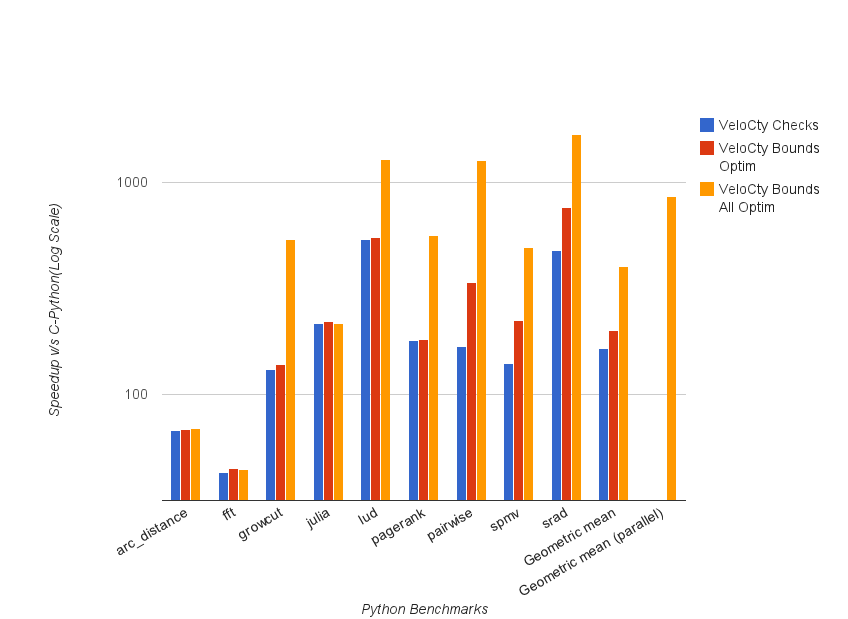
\includegraphics[scale=0.5]{Figures/final_py.png}
\caption[Summary of Python Results]{The bar graph gives the speedups of the \velocty backend for diferent \velocty versions compared to the Mathworks' JIT and VM implemenation. Higher is better. Geometric mean(parallel) gives the speedups of the 6 benchmarks that can be executed in parallel. }
\label{fig:results_final}
\end{figure}

Similar to \matlab we can see the geometric mean of the \velocty versions increasing as we add optimisations. The geometric mean of the baseline \velocty version is 164.48x , the geometric mean of the version with bounds check optimisations enabled is 200.8x and the geometric mean when \velocty code is executed in parallel is 400.98x. The geometric mean of benchmarks which are executed in parallel is 860.09x.

Note that since none of the Python benchmarks contained any array slicing operations or array operations, performance would not differ when the memory optimisation was used and hence we do not specify those numbers in this section. 
\section{Summary}
Through our experiments we showed that compiling `hot' functions of \matlab and Python show significant performance improvement. 
For the \matlab benchmarks, we observed significant  speedups compared to the Mathworks' \matlab interpreter and JIT compiler. We also observed comparable performance with respect to \matlab-coder. We identified bottlenecks in generated code and implemented optimsations, namely the bounds check elimination and the memory optmisation to reduce the impact of the bottlenecks. Due to these optimisations we also observed significant speedups over \matlab-coder for most benchmarks. Moreover we also identified the bottlenecks in the benchmarks which showed poorer performance compared to \matlab-coder and suggested optimisations to eliminate the bottlenecks. The generated code showed significant performance gains for three benchmarks when it was executed in parallel using OpenMP.

On the Python side, we saw very large speedups against the C-Python interpreter. The larger speedup could be attribute to the fact that comparison was against an interpreter without a JIT compiler. We also observed equal or better performance when compared to Cython. The performance of the generated code improved further when the optimisations were added and the code was executed in parallel. 

In conclusion, the VeloCty code with all optimisations enabled generated by \velocty from \matlab is 8.05 times faster than the Mathwork's \matlab. The generated VeloCty code for Python is 400.98 times faster than the C-Python interpreter. We believe that these results are encouraging and have motivated us to further develop the compiler for higher performance gains. 
